\chapter{Podstawy teoretyczne}

Problem kategoryzacji obrazów wpisuje się w dziedzinę rozpoznawania obrazów. Zadanie to polega na rozpoznaniu przynależności różnych rodzajów obiektów do pewnych klas\cite{Tad91} i jest częścią większego zagadnienia, które określa się jako uczenie maszynowe.

\section{Uczenie maszynowe}

Uczenie maszynowe jest zagadnieniem interdyscyplinarnym z pogranicza informatyki, statystyki i sztucznej inteligencji, które zajmuje się tworzeniem systemów mogących doskonalić się za pomocą dostarczanych danych.

Systemy te ulegają nieustannej modyfikacji, zmieniają swoje wewnętrzne parametry po to by osiągnąć korzyści takie jak zwiększenie efektywności lub wydajności działania. Ważną cechą jest to, że jakkolwiek zmiany te zachodzą na podstawie czynników zewnętrznych to jednak dokonują się w~systemie autonomicznie. System, który się uczy zmienia sam siebie na lepsze.\cite{CICHOSZ00}

\section{Uczenie nadzorowane i nienadzorowane}

W uczeniu maszynowym możemy wyróżnić dwa zasadnicze podejścia: uczenie nadzorowane (\emph{ang. supervised machine learning}) i nienadzorowane (\emph{ang. unsupervised machine learning}). Różnica pomiędzy nimi polega na obecności w uczeniu nadzorowanym tzw. nauczyciela, który stanowi źródło informacji trenującej. Posługując się analogiczną terminologią, system który podlega nauce określa się jako ucznia. Na rys. \ref{fig:supervised-learning} przedstawiono schemat uczenia maszynowego z użyciem nauczyciela.

\begin{figure}[h]
	\centering
	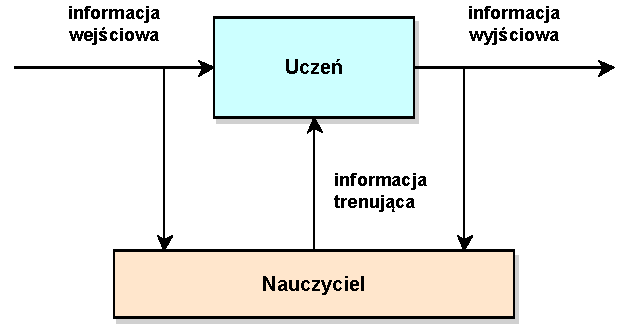
\includegraphics{graphics/01_podstawy_teoretyczne/supervised-learning.pdf}
	\caption{Uczenie maszynowe z nauczycielem \cite{CICHOSZ00}}
	\label{fig:supervised-learning}
\end{figure}

Uczeń otrzymuje od nauczyciela informację o tym jakiego komunikatu wyjściowego oczekuje w odpowiedzi na przykładowe informacje wejściowe. Mogą być one dostarczone np. w formie par składających się z wektorów danych oraz poprawnej odpowiedzi: $(x_{i}, y_{i})$. Na podstawie przykładów, system ma wyuczyć się przyporządkowywania danych do odpowiednich odpowiedzi. Innymi słowy, ma nauczyć się takiej funkcji $f$, dla której $f(x_{i})=y_{i}$, dla każdego $i$. Przykładami w uczeniu maszynowym mogą być różne obiekty, takie jak przedmioty, osoby, obserwacje.

Każdy przykład określany jest przez skończony oraz niepusty zbiór atrybutów $A=\lbrace a_{i}, a_{2}, ..., a_{n}\rbrace$. Atrybuty ze względu na rodzaj dziedziny możemy podzielić na: 
\begin{compactitem}
	\item nominalne, tj. takie, których dziedziny są zbiorami nieuporządkowanymi - dla dwóch wartości możliwe jest określenie jedynie czy są równe czy nierówne,
	\item porządkowe, dla których dziedziny są zbiorami uporządkowanymi, czyli możliwe jest określenie relacji porządku liniowego na zbiorze wartości,
	\item liczbowe, których dziedziny są zdefiniowane jako zbiór liczbowy.
\end{compactitem}

W zależności od rodzaju odpowiedzi możemy wyróżnić dwa typowe rodzaje problemów, które stara się rozwiązać uczenie nadzorowane. Jeśli system ma przyporządkować do wektora wejściowego pojedynczą kategorię pochodzącą ze skończonego i dyskretnego zbioru kategorii, wówczas określamy ten problem jako problem kategoryzacji. Natomiast w przypadku przyporządkowywania odpowiedzi składającej się z jednej lub więcej zmiennych ciągłych, mówimy o problemie regresji.\cite{BISHOP06} Proces działania maszyny realizującej uczenie nadzorowane możemy podzielić na dwa etapy: etap treningu lub też nauki oraz etap polegający na rozwiązywania przynależności nowych wektorów wejściowych, który często określa się jako testowanie lub walidację.

W uczeniu nienadzorowanym nie występuje rola nauczyciela, a co za tym idzie, do systemu nie trafiają informacje treningowe. Dostępne są jedynie wektory wejściowe i na podstawie ich obserwacji system ma nauczyć się odpowiednich odpowiedzi.\cite{CICHOSZ00} Podejście to nie polega zatem na przyporządkowaniu wektorów do ustalonych wcześniej kategorii, lecz na wyznaczeniu ukrytej struktury w danych, które są nieopisane.\cite{VALPOLA} Wykorzystywane jest m.in. do rozwiązywania problemu klasteryzacji (\emph{ang. clustering}), który polega na znajdowaniu grup podobnych obiektów wśród danych wejściowych. Ponadto uczenie nienadzorowane wykorzystywane jest to określania rozkładu danych w przestrzeni wejściowej, co nazywamy szacowaniem rozkładu (\emph{ang. density estimation}) lub do rzutowania danych z przestrzeni wielowymiarowej do trójwymiarowej w celu dokonania wizualizacji.\cite{BISHOP06}

Na rys. \ref{fig:unsupervised-learning} przedstawiono uproszczony schemat mechanizmu uczenia nienadzorowanego. Algorytm uczący dokonuje podziału zestawu danych na klastry, które następnie muszą zostać zinterpretowane przez człowieka. W zaprezentowanym przykładzie klastry zostały nazwane na podstawie analizy ich zawartości. W rzeczywistych problemach zadanie nadania etykiet wytworzonym klastrom może okazać się trudne i może wymagać dostrojenia parametrów algorytmu by identyfikacja klastrów była możliwa.

\begin{figure}[h]
	\centering
	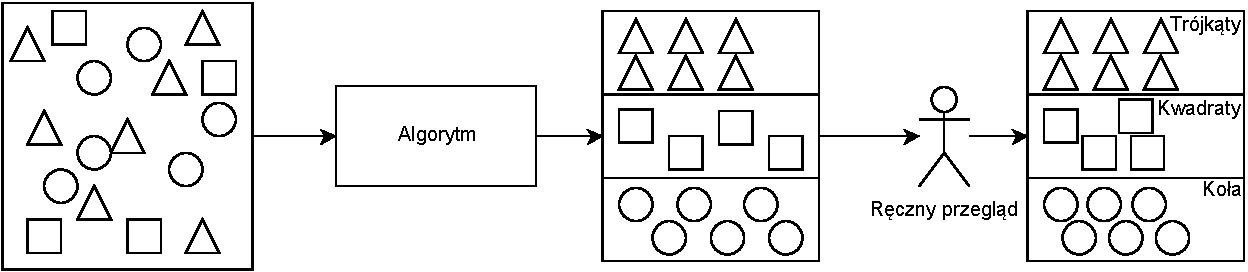
\includegraphics[scale=0.8]{graphics/01_podstawy_teoretyczne/unsupervised-learning.pdf}
	\caption{Uczenie maszynowe nienadzorowane \cite{CASEY}}
	\label{fig:unsupervised-learning}
\end{figure}

Dane wejściowe z etapu walidacji mogą się różnić od przykładowych danych służących do wytrenowania systemu. Umiejętność udzielania poprawnej odpowiedzi na komunikaty, które różnią się od przykładowych danych określamy jako generalizacja.\cite{BISHOP06}
%TODO napisac o tym w kontekscie pracy, co raczej sie nadaje a co raczej nie

\section{Rozpoznawanie wzorców}
Celem rozpoznawania wzorców (\emph{ang. pattern recognition}) jest stworzenie symbolicznego opisu dla zawartości jedno lub wielowymiarowego sygnału cyfrowego takiego jak np. cyfrowy obraz graficzny, sygnał mowy, lub obraz z kamery, a następnie przyporządkowanie do niego klasy lub instancji klasy. Opis ten może być zrealizowany w różnej formie: funkcji, obiektów, ruchu, wyrazów lub struktur.

Wzorcem nazywamy zbiór cech, który tworzy ilościowy oraz jakościowy opis obiektu. Wzorzec zapisujemy najczęściej jako wektory, ciągi lub drzewa. Wzór \ref{pattern_vector} przedstawia wektor wzorca, gdzie $x_{i}$ reprezentuje $i$-tą cechę, a $n$ oznacza ilość wszystkich cech powiązanych ze wzorcem.\cite{GONZALES01}

\begin{equation} 
\label{pattern_vector} 
\overrightarrow{x}=
\begin{bmatrix}x_1\\
x_2\\
\vdots\\
x_n  
\end{bmatrix}
\end{equation}

Zbiór wzorców charakteryzujący się podobnymi wektorami cech nazywamy klasą wzorców i oznaczamy jako $\omega_1, \omega_2, ..., \omega_{W}$, gdzie dolny indeks określa numer klasy, a $W$ określa ilość klas. Jako rozpoznanie wzorca $\omega$ określa się przyporządkowanie wzorcowi jego klasy.

W systemach analizy sygnałów możemy oprócz rozpoznania zdefiniować również dwa inne pojęcia: identyfikację oraz weryfikację. Zazwyczaj gdy nie dysponujemy opisami klas wzorców, a jedynie przechowujemy wzorce referencyjne, celem systemu jest porównanie aktualnego wzorca z bazą referencyjną. Jeśli na podstawie określonej odległości pomiędzy parami wzorców system jest w stanie dokonać wyboru dokładnie jednego wzorca referencyjnego, to określamy takie rozwiązanie jako identyfikację. Natomiast jeśli możemy wybrać przynajmniej jeden ze wzorców referencyjnych to określamy takie rozwiązanie jako weryfikację.




\section{Selekcja cech}


\section{Ekstrakcja cech}
%TODO problem ograniczania wielkosci wektora cech
%TODO podac przyklady z literatury jak robiono ekstrakcje poprzednio
...

\section{Klasyfikacja}
%TODO wymienic rozne rodzaje klasyfikatorow
%https://www.youtube.com/watch?v=qdDHp29QVdw
...


\subsection{Klasyfikator według funkcji potencjału}
...
	
\subsection{Klasyfikator statystyczny Bayesa}
...
	
\subsection{Klasyfikator według minimalnej odległości}
...
	
\subsection{Klasyfikator k Najbliższych Sąsiadów}
...

\subsection{Maszyna wektorów wspierających (SVM)}
...
	
\section{Ocena klasyfikatorów}
...

%\section{Porównanie klasyfikatorów}